\section{Text Aggregation Graphs}
\label{sec-cl2017:tag}

\begin{figure}[t!]
\begin{center}
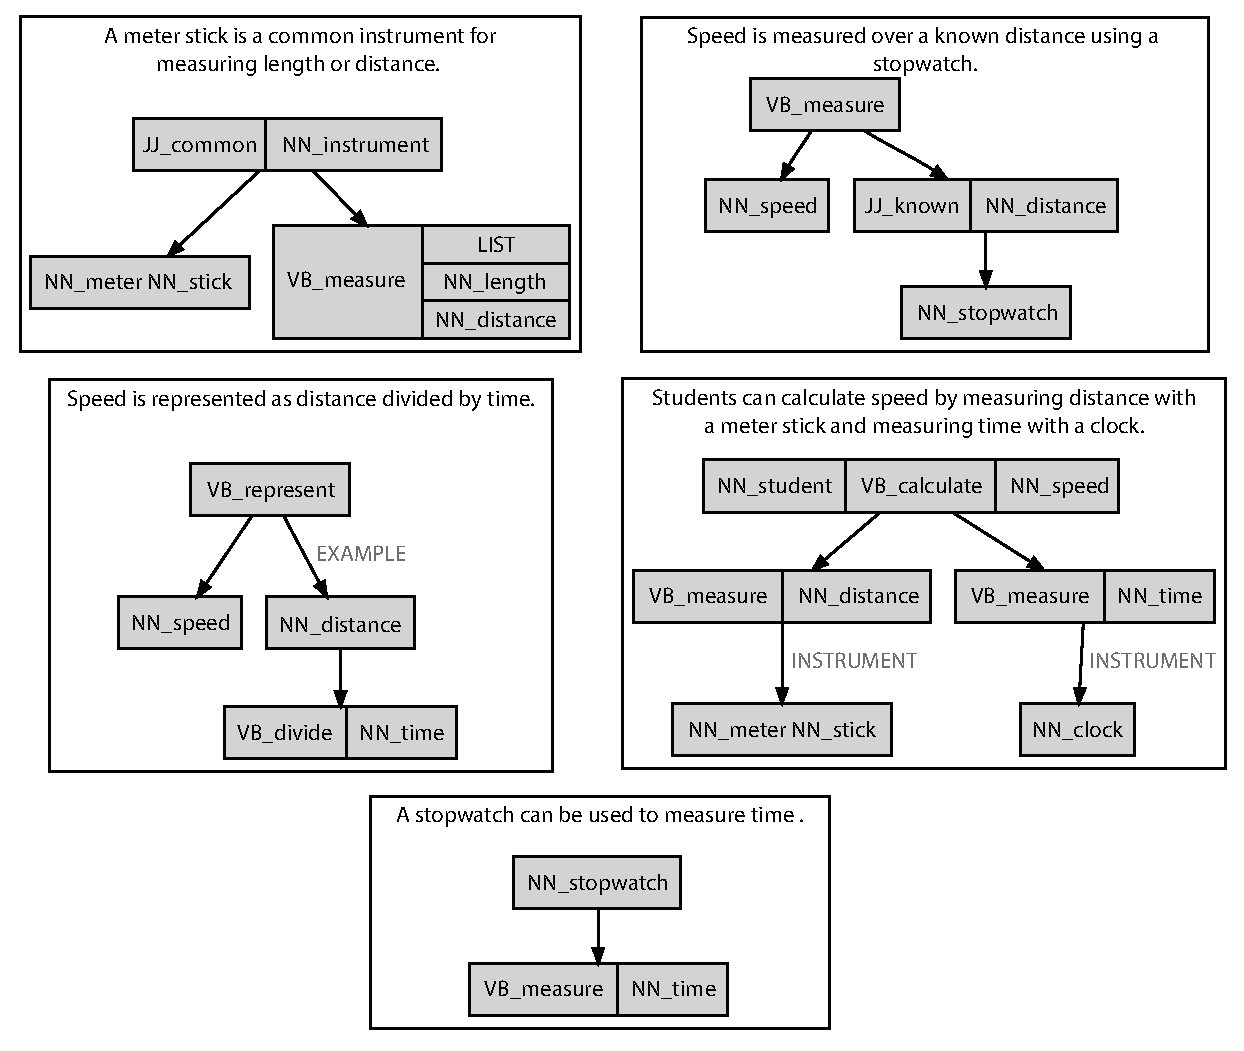
\includegraphics[width=\textwidth]{mainmatter/tacl2015-tig/example_graphlets1.pdf}
%	\centering
%	\begin{minipage}[b]{0.4\textwidth}	
%		\includegraphics[scale=0.4]{meter_length_distance.pdf}
%	\end{minipage}
%	\hfill
%	\begin{minipage}[b]{0.4\textwidth}	
%		\includegraphics[scale=0.4]{speed_distance_stopwatch.pdf}
%	\end{minipage}
%
%
%	\begin{minipage}[b]{0.4\textwidth}	
%		\includegraphics[scale=0.4]{speed_distance_time.pdf}
%	\end{minipage}
%	\hfill
%	\begin{minipage}[b]{0.4\textwidth}	
%		\includegraphics[scale=0.4]{speed_meter_clock.pdf}
%	\end{minipage}
\end{center}	
%space{-2mm}
\caption{Five example graphlets for five sentences that could be aggregated together in different combinations to justifiably answer the question \emph{What tools could determine the speed of turtles walking along a path? (Answer: stopwatch and meter stick)}.  Each graphlet contains one or more information nuggets (grey boxes) composed of one or more terms.  For example, the graphlet for the sentence \emph{A stopwatch can be used to measure time} contains two information nuggets.  Edges between nuggets within a graphlet are shown with arrows, where a subset of these edges are labelled (e.g., \emph{EXAMPLE, INSTRUMENT}), and the rest are unlabelled. 
}
%space{-5mm}
\label{fig:conceptexamples}
%\end{center}
\end{figure}

In order to answer complex questions requiring inference, we propose a method for aggregating information from multiple knowledge base sources to form multi-sentence justifications that link questions to their answers.  These human-readable justifications additionally provide a form of interpretability to the model, allowing the human user to see what the model considers important in identifying correct answers as well as where the model goes wrong.  When constructing these justifications, there is a risk of drifting to semantically unrelated concepts and so while we aggregate at the word-level (to maintain robustness), we qualify the aggregation using sentence-level context (to maintain context). 

To achieve this, we represent our knowledge base sentences as lightly-structured graphs, which we call \textbf{graphlets}, and then aggregate them together based on lexical overlap to form our justifications.  The graphlet nodes contain sentence text and the edges capture the syntactic dominance between nodes as well as certain specialized roles (e.g., \emph{instrument} and \emph{cause}), in the form of sparse edge labels.  Example sentences and corresponding graphlets are shown in Figure \ref{fig:conceptexamples}.  Below is a description of how we build our graphlets and then assemble them into our multi-sentence justifications, but for more detail, please see \citet{jansen2017framing}.
%The representation is intended to strike a balance between structure and robustness -- i.e., to include enough context in each of the nodes to mitigate semantic drift, while still representing the underlying syntactic structure of the text.  In this way, these graphlets can be construed as a middle ground between free-text and the dependency-syntax graph.

We build our graphlets in two stages.  We first decompose knowledge base sentences into smaller units (along clausal and prepositional boundaries) which we call \textbf{information nuggets} \citep{Voorhees:2003}.  These smaller units reduce the sparsity of the whole sentence while still maintaining clausal context.  Then we connect sentence nuggets together if any of their words were originally linked through syntactic dependencies.  Formally, we use the following algorithm:

\begin{enumerate}
\item \textbf{Syntactic parsing:} The text is syntactically parsed using the sentences using the Stanford CoreNLP toolkit \citep{manning2014stanford}.  

\item \textbf{Decompose sentence into information nuggets:} The dependency graph is used to decompose the sentence into information nuggets (i.e., the graphlet nodes) by segmenting along specified dependencies that represent clausal complements ({\tt ccomp, xcomp}), adverbial and relative clause modifiers ({\tt advcl, rcmod}), reduced non-finite verbal modifiers ({\tt vmod}), and certain empirically determined prepositional phrases (e.g., \texttt{prep\_with}, etc.)\footnote{The full list of prepositional dependencies along which we split is: {\tt prep\_with, prep\_through, prep\_from, prep\_to, prep\_as, prep\_into, prep\_by, prep\_in, prep\_such\_as, prep\_because\_of, prep\_over, prep\_on, prep\_between, prepc\_as, prepc\_by, prepc\_of, prepc\_with, prepc\_after, prepc\_for, prepc\_before, prep\_before, prep\_after, prep\_during, prepc\_during, prepc\_because\_of, prep\_without,} and {\tt prepc\_without}.}.  The text within the node is segmented into terms, i.e. one or more words.  While the default is one word, a term may contain a noun-noun compound or a comma-separated list.  

\item \textbf{Construct graphlets:} These nuggets are then connected by edges whenever there is an outgoing dependency from one nugget to another.  The edges are labeled as either \texttt{instrument, process, example, temporal, contrast}, or \texttt{unknown}, with the vast majority being labeled as \texttt{unknown}.  These labels are assigned based on specified dependency links (i.e. the dependency link \texttt{prep\_such\_as} corresponds to the label \texttt{example}).\footnote{More specifically, in our method the {\tt instrument} label corresponds to the dependencies {\tt prep\_with, prep\_through}, and {\tt prep\_by}.  The label {\tt process} corresponds to the dependencies {\tt prep\_from, prep\_to, prep\_into, prep\_because\_of}, and {\tt prepc\_because\_of}.  The {\tt example} label corresponds to {\tt prep\_as, prepc\_as, prep\_such\_as}, and {\tt prepc\_such\_as}.  The {\tt temporal} label corresponds to {\tt prep\_before, prepc\_before, prep\_after, prepc\_after, prep\_during} and {\tt prepc\_during}.  Finally, the {\tt contrast} label corresponds to {\tt prep\_without} and {\tt prepc\_without}.}

\item \textbf{Remove stop words}: Finally, stop words as well as words that are not nouns, verbs, or adjectives are removed.

\end{enumerate}



%Semantic drift, or the tendency for a graph traversal to drift to unrelated topics,
%constitutes a major hurdle for lexical semantic QA models.  
%This was noted recently by Fried et al.~\citeyear{fried2015higher}, who proposed an approximation of inference for QA as the traversal of a graph that connected concepts (words or lexicalized syntactic dependencies) along lexical semantic associations. While this method is robust and performs better than approaches relying on alignment or embedding models alone, it does not have a good way of keeping an inference on-context when traversing the concept association graph.
%Moreover, even when a correct answer is selected, these methods operate on sets of probabilities over word distributions, and are unable to provide a compelling human-readable explanation to the user as to why a given answer is correct. 
%
%To address these issues, we propose to construct multi-sentence answer justifications using a  sentence aggregation method that combines the robustness of word-level connections with sentence-level context.  
%Our approach works in two steps, both of which are performed offline, i.e., before the actual QA process. First, we decompose sentences that are likely to justify science exam answers (e.g., from knowledge bases such as study guides) into smaller units based on clausal and prepositional phrase boundaries. Intuitively, this allows us to maintain sufficient context to control semantic drift, while, at the same time, mitigating the sparsity of complete sentences.  
%Following previous QA terminology, we call these smaller units,  which represent clauses or prepositional phrases, {\bf information nuggets}~\cite{Voorhees:2003}. We connect two information nuggets within the same sentence if there are any syntactic dependencies that connect any words in these nuggets. We call the resulting graph of these information nuggets, which represents an entire sentence, a \textbf{graphlet}. 
%Figure \ref{fig:conceptexamples} shows a number of example graphlets. 
%Formally, we transform sentences into graphlets using the following algorithm:
%
%
%\begin{enumerate}
%
%\item{\textbf{Parse knowledge base sentences: } 
%All knowledge base sentences are syntactically parsed using the Stanford CoreNLP toolkit~\cite{manning2014stanford}.}
%
%% ms: let's use {\tt } for syntactic dependencies, and {\em } font for text.
%
%\item {\textbf{Decompose sentences into information nuggets: \label{step:creatinggraphlets}} 
%For each sentence, beginning at the root of the dependency graph, we traverse the dependency graph and segment the sentence into nuggets along clausal complements ({\tt ccomp, xcomp}), adverbial and relative clause modifiers ({\tt advcl, rcmod}), reduced non-finite verbal modifiers ({\tt vmod}), and a subset of empirically determined prepositional phrases.\footnote{The full list of prepositional dependencies along which we split is: {\tt prep\_with, prep\_through, prep\_from, prep\_to, prep\_as, prep\_into, prep\_by, prep\_in, prep\_such\_as, prep\_because\_of, prep\_over, prep\_on, prep\_between, prepc\_as, prepc\_by, prepc\_of, prepc\_with, prepc\_after, prepc\_for, prepc\_before, prep\_before, prep\_after, prep\_during, prepc\_during, prepc\_because\_of, prep\_without,} and {\tt prepc\_without}.}
%}
%
%\item {\textbf{Segment nuggets into terms: }
%Each nugget is segmented into one or more terms.  A term is nominally a single word, but we join both noun compounds and lists into single terms.  Noun compounds (e.g., \emph{meter stick} in Figure \ref{fig:conceptexamples}) are detected using the {\tt nn} dependency tag, and lists of words (e.g., \emph{sleet, rain, hail, or snow}) are detected through the same patterns used by the focus word extractor (see Section \ref{sec-cl2017:focuswords}).
%}
%
%
%\item {\textbf{Construct graphlets:} Two nuggets within a graphlet are connected if any of the words in one nugget have links in the syntactic dependency tree with words in the other nugget. } 
%
%\item {\textbf{Label a subset of the graphlet  edges:} In general, to increase robustness, edges between nuggets are unlabelled.  The exceptions to this are a small set of high-confidence labels: the label {\tt definition} derived from the semi-structured dictionary resources which distinguish between a defined word and its definition, and the labels {\tt instrument, process, example, temporal}, and {\tt contrast} derived from prepositional dependencies.\footnote{More specifically, in our method the {\tt instrument} label corresponds to the dependencies {\tt prep\_with, prep\_through}, and {\tt prep\_by}.  The label {\tt process} corresponds to the dependencies {\tt prep\_from, prep\_to, prep\_into, prep\_because\_of}, and {\tt prepc\_because\_of}.  The {\tt example} label corresponds to {\tt prep\_as, prepc\_as, prep\_such\_as}, and {\tt prepc\_such\_as}.  The {\tt temporal} label corresponds to {\tt prep\_before, prepc\_before, prep\_after, prepc\_after, prep\_during} and {\tt prepc\_during}.  Finally, the {\tt contrast} label corresponds to {\tt prep\_without} and {\tt prepc\_without}.}}
%
%\item {\textbf{Remove stop-words:}  Finally, we remove any stop words, as well as words that are not nouns, verbs, or adjectives.  Any nuggets that are empty after this filtering are removed. }
%
%\end{enumerate}

\begin{figure}[t!]
\begin{center}

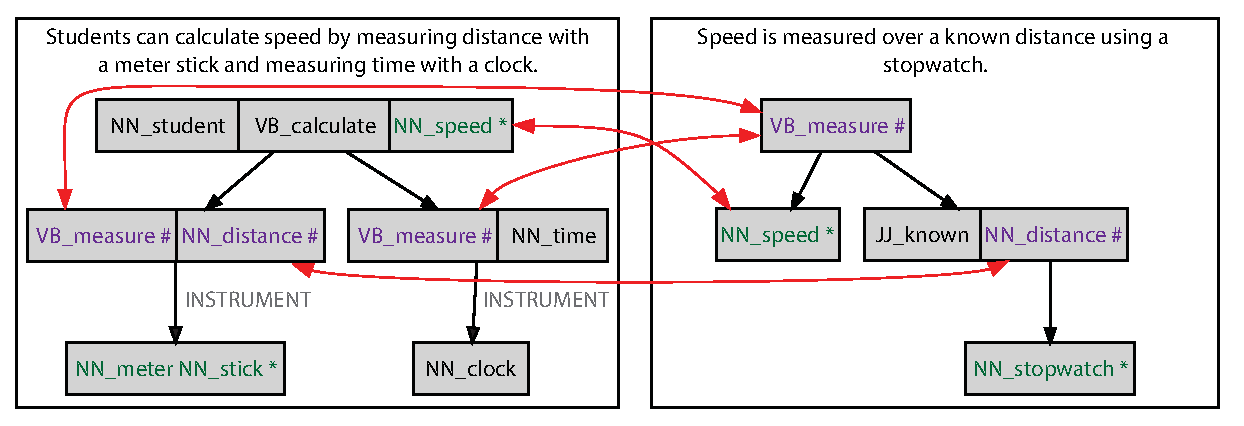
\includegraphics[width=\textwidth]{mainmatter/tacl2015-tig/tag_connection_example2.pdf}
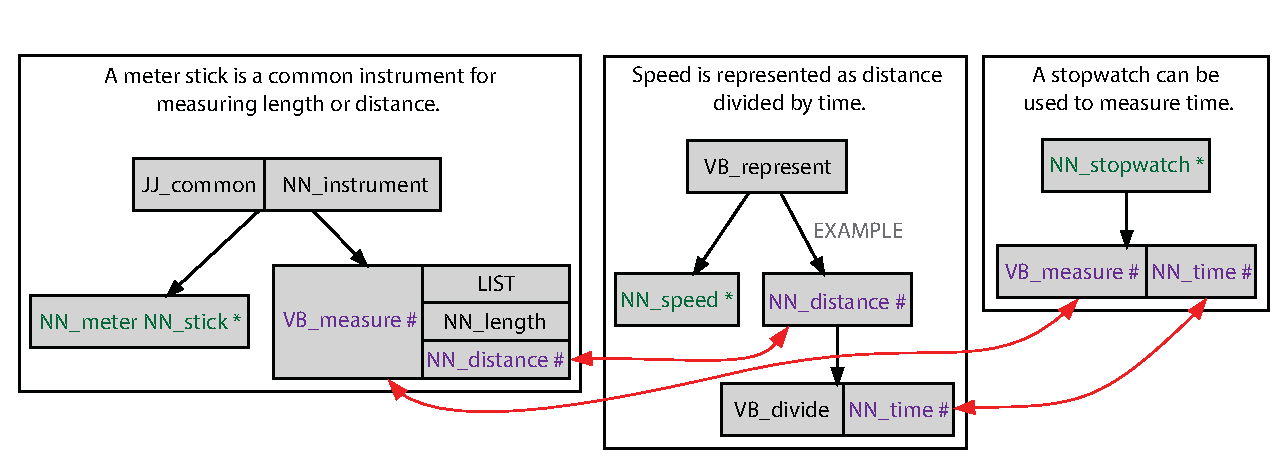
\includegraphics[width=\textwidth]{mainmatter/tacl2015-tig/tag_example2.pdf}

%space{-2mm}
\caption{
Two example Text Aggregation Graphs (TAGs) that justifiably answer the question \emph{What tools could determine the speed of turtles walking along a path} for the answer \emph{a stopwatch and meter stick}. Asterisks (*) denote that a given term is either a question or answer focus word, while pounds (\#) denote terms that are not found in the question or answer, but which are shared between graphlets.  Links between the graphlets in a given TAG are highlighted. (top) A two-sentence TAG, where the edges between graphlets connect on a focus word \emph{(speed)} and other words shared between the graphlets \emph{(distance, measure)}. (bottom) A three-sentence TAG, where the edges between graphlets connect entirely on shared words between the graphlets \emph{(distance, measure, time)} that are not focus words.
}
%space{-5mm}
\label{fig:tag_example}
\end{center}
\end{figure}

%\subsection{Assembling graphlets into justifications}

Once we have created the graphlet representations of our knowledge base sentences, we connecti sentence graphlets that have any lexical overlap between their nuggets.  The resulting, joined graph structure we call a \textbf{text aggregation graph (TAG)} and this TAG serves as a potential answer justification.\footnote{While conceivably we could construct TAGs of any length, currently we allow our TAGs to consist of up to three graphlets.}
Figure~\ref{fig:tag_example} shows an example of two TAGs. 
We make use of the multiple levels of TAG structure (clausal, sentence, and intersentence) when designing features that characterize the TAG in terms of its fitness in serving as a justification for a given answer (see Section \ref{sec-cl2017:scoring}).

%After the sentences have been transformed into graphlets, we construct candidates for multi-sentence justifications by connecting sentences with any lexical overlap between information nuggets.  We currently connect up to three graphlets into constructs we call \textbf{text aggregation graphs (TAGs)}, where each TAG corresponds to one potential answer justification. 
%Figure~\ref{fig:tag_example} shows an example of two TAGs. 
%Note that a TAG contains multiple levels of structure: (a) clause-level structure within nuggets, (b) sentence-level structure within graphlets, and (c) intersentence structure within TAGs\footnote{Currently, the graphlets and TAGs make use of lexical and syntactic structure only.  While this provides a robust representation of much of the structure in text, in a future system we would also like to explore adding semantic role and discourse information in our graphlets. Both of these have been shown to be useful, albeit for simpler QA tasks~\cite{Surdeanu:11,jansen14}.}.  
%We will exploit this information in the next section, where we design features to capture the fitness of a TAG as a justification for a given answer.



\section{Text Aggregation Graph Features}
\label{sec-cl2017:scoring}

Once candidate answer justifications have been reframed as text aggregation graphs, the TAGs for each answer candidate need to be ranked such that a good justification for the correct answer will be ranked above all other answer justifications for incorrect answers. We describe the features that we extract from TAGs for this ranking in this section, and the latent ranking algorithm in Section~\ref{sec-cl2017:perceptron}.




\begin{table}[]
\footnotesize{
\begin{tabular}{p{35mm}p{105mm}}
\hline
Feature & Description \\
\hline
\multicolumn{2}{l}{\emph{TAG-level features:}} \\
%numFocus			&	Number of unique Q and A focus words present in the TAG					\\
numFocusQ			&	Number of unique Q focus words present in the TAG						\\
numFocusA			&	Number of unique A focus words present in the TAG						\\
massFocusQ			&	Sum of the unique Q focus word weights present in the TAG				\\
massFocusA			&	Sum of the unique A focus word weights present in the TAG				\\
%\\
%\multicolumn{2}{l}{\emph{Other TAG-level Scores:}} \\
numRepeatedFocus	&	Number of focus words contained in more than one graphlet, with repetition \\
numOtherAnswerF		&	Negative predictor: the number of focus words from other multiple choice answers included in the current TAG.	\\
minConcShared		&	The minimum psycholinguistic concreteness score (i.e., abstractness) of any shared word in the TAG \\
\\
\multicolumn{2}{l}{\emph{Nugget-level features: }} \\
numNugF				&	Number of nuggets that are entirely focus words. \\
numNugFS 			&	Number of nuggets that contain only focus words and shared words. \\
numNugFSO			&	Number of nuggets that contain focus, shared, and other unmatched words. \\
numNugFO			&	Number of nuggets that contain only focus words and other words. \\
numNugS				&	Number of nuggets that contain only shared words. \\
numNugSO			&	Number of nuggets that contain only shared words and other words. \\
numNugO				&	Number of nuggets that contain only other words. \\
% \\
% \multicolumn{2}{l}{\emph{Other Nugget-level features: }} \\
numDefinedFocus		&	Number of nuggets containing only focus words with outgoing {\tt definition} edge \\
numDefinedShared	&	Number of nuggets containing only shared words with outgoing {\tt definition} edge \\
numQLinksFocus		&	Number of nuggets containing only focus words that have an incoming labeled link (e.g., {\tt definition, instrument, process, temporal})  \\
numQLinksShared		&	Number of nuggets containing only shared words that have an incoming labeled link  \\
numNuggetMultiF		&	Number of nuggets that contain more than one focus word\\
\\
\multicolumn{2}{l}{\emph{Bridge features:}} \\
massMaxBridgeScore		&	Bridge graphlets are graphlets that contain at at least one focus word from both the  \\
massMinBridgeScore		&	question and answer, signifying that they are highly relevant to the question and the \\
massDeltaBridgeScore	&	corresponding answer. A   graphlet's bridge score is the sum of this focus word mass.  We calculate the minimum, maximum, and delta (max $-$ min) bridge scores across all graphlets within a TAG. \\
\\
\hline
\end{tabular}
}
\caption{{  Features used to score candidate answer justifications represented as TAGs. }} 
\label{tab:features}
\end{table}


\subsection {Features} 
\label{sec-cl2017:featuresandscoring}

We developed a set of TAG features that capture both the type of connections between the graphlets in a TAG, and how well the TAG as a whole relates to the corresponding question--answer pair.
The features can be broadly grouped into count features and mass features. Count features count the integer number of instances of a given event in a TAG -- for example, the number of nuggets that are entirely focus words.  Mass features sum the weights of focus words (as computed in Section~\ref{sec-cl2017:focuswords}) -- for example, summing the weight of all question or answer focus words found either within a single graphlet, or across the entire TAG.

A full list of the features and their descriptions can be found in Table \ref{tab:features}.
%
The features are grouped into three categories: TAG-level, nugget-level, and bridge features. 
The TAG-level features use focus words to evaluate the likelihood that an entire justification is relevant to the question and answer candidate. 
Nugget-level features provide a finer-grained measure of how well the individual sentences in a justification relate to each other by quantifying both \emph{how fully} they are connected (e.g., are all the words in a nugget matched with words in other nuggets, or only some), and what type of words they connect on (e.g., \emph{focus words}, or \emph{other words} not found in the question but shared between sentences).
Separate features encode whether a nugget is all focus words, all shared words, all unmatched words, or any partial combination of these three categories.
Finally, we define a graphlet that contains both question and answer focus words as a \emph{bridge graphlet}, in that its content tends to span or \emph{bridge} the question and answer, and include a set of bridge features for evaluating this subset of highly-relevant graphlets. 




%- TAG = path = answer justification
\begin{figure}[t!]
\begin{center}
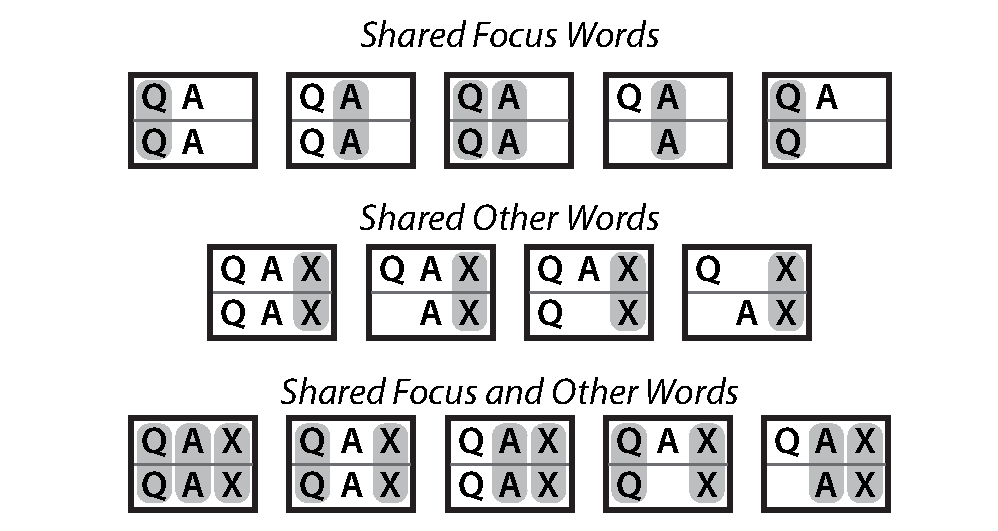
\includegraphics[width=100mm]{mainmatter/tacl2015-tig/connection_types.pdf}
%space{-2mm}
\caption{{Connections between sentences are characterized based on lexical overlap between graphlets.
Here, each box represents a two-sentence TAG, with graphlets stacked vertically.  The presence of question or answer focus words is marked with \emph{Q} or \emph{A}, while the presence of other non-focus words shared between the two graphlets is marked with \emph{X}.  Lexical overlap within a category is highlighted.
}}
%space{-5mm}
\label{fig:connectiontypes}
\end{center}
\end{figure}


\subsection {Modeling Different TAG Types Using Domain Adaptation} % Characterizing Lexical Overlap Between Sentences}
\label{sec-cl2017:characterizing}

Good justifications for an answer may take a variety of forms, from those with little lexical overlap due to the ``lexical chasm''~\citep{Berger:00} between question and answer, to those with a great deal of overlap. For example, of the two TAGs shown in Figure~\ref{fig:tag_example}, in the first TAG both sentences connect on question focus words, while in the second TAG the graphlets only connect on other non-focus words. 

Understanding the connections between sentences in a TAG serves as a robust proxy to modeling discourse structures (e.g., whether the second sentence elaborates on the concepts introduced in the first), which has been previously shown to increase both open-domain and science-domain QA performance~\citep{jansen14}.
This is important in the context of feature representations, because we conjecture that some features may be important across all the ways a justification can connect (so these features should be jointly modelled across connection types), whereas others are specific to certain connection types (so they should be modeled separately by type). As shown in Section~\ref{sec-cl2017:experiments}, this hypothesis is strongly empirically supported.

To model this phenomenon, we adapt a technique from the field of domain adaptation~\citep{daume2007}.
First, we label each of the sentences within a TAG based on whether they contain question focus words and/or answer focus words.  We then characterize the entire TAG by determining whether the words shared between sentences are question focus words, answer focus words, or other non-focus words.  This leads to 14 possible connection types, depicted in Figure \ref{fig:connectiontypes}.\footnote{In practice, for a configuration that allows TAGs of 1 or 2 sentences, we have 15 connection types, including the 14 two-sentence connection types, plus a single-sentence type. We ignore the single-sentence type in this discussion for simplicity, though it is included in our model.}
Second, following Daum{\'e}'s method, we generate 15 versions for each of the features introduced in Section~\ref{sec-cl2017:featuresandscoring}: a generic one that is type independent, and 14 that are affixed by each of the connection types. For example, for a given feature such as \emph{numFocusQ}, we create 15 copies: \emph{numFocusQ, numFocusQ$_1$ ... numFocusQ$_{14}$}, where the subscript (when present) indicates a specific connection type. For a TAG of connection type \emph{i}, only values for the type-specific feature \emph{numFocusQ$_i$} as well as the general feature \emph{numFocusQ} are populated -- all other \emph{numFocusQ$_j$} features are set to a value of zero. This allows the learning algorithm in the next section to learn whether each feature generalizes across connection types, or not. As shown in~\citet{finkel2010hierarchical}, this approach is equivalent to a joint model with a hierarchical prior. 



While the features introduced in Table~\ref{tab:features} apply to justifications containing any number of sentences, characterizing justifications that are longer than two sentences is not straightforward, as the number of connection types (Figure~\ref{fig:connectiontypes}) would become prohibitively large.   We handle three-sentence justifications by treating each as a set of three two-sentence TAGs, and characterize each two-sentence connection individually.  In the case where two groups of sentences have the same connection type, we take the highest scoring version of each overlapping feature.  While this method would extend to justifications of arbitrary length,  justifications longer than three sentences are not currently generated by our system. 


